\section{ParticipantRole}
\label{sec:ParticipantRole}
%%%%%%%%%%%%%%%%%%%%%%%%%%%%%%%%%%%%%%%%%%%%%%%%%%%%%%%%
\begin{figure}[h!]
\begin{center}
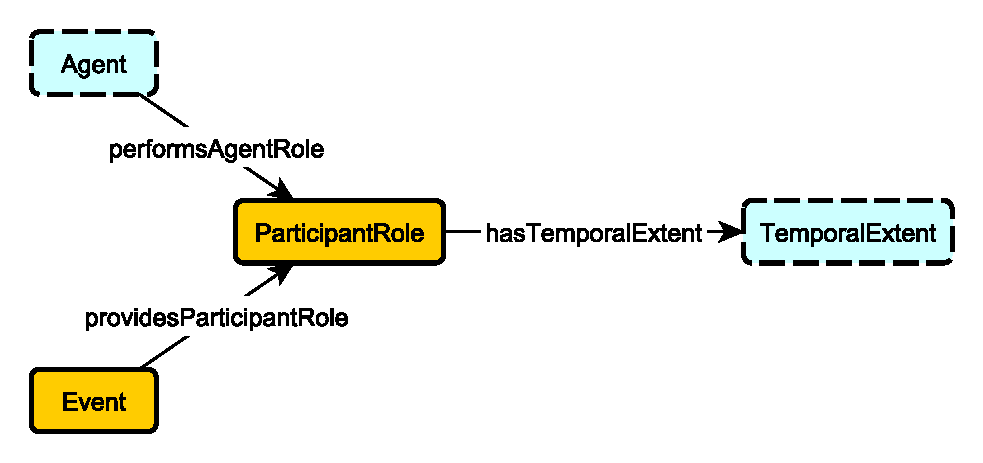
\includegraphics[width=.8\textwidth]{figures/participantrole}
\end{center}
\caption{Schema Diagram for the ParticipantRole Pattern. The visual notation is explained in Chapter \ref{chap:prelims}.}
\label{fig:ParticipantRole}
\end{figure}
\subsection{Summary}
\label{sum:ParticipantRole}
%%%%%%%%%%%%%%%%%%%%%%%%%%%%
The \textsf{ParticipantRole} Pattern is a specialization of the \textsf{AgentRole} Pattern, which can be found in Section \ref{sec:AgentRole}; many axioms are inherited due to this. We include it for convenience as it occurs frequently in our modelling experiences. This pattern has additional synergies with the \textsf{Event} Pattern \cite{event,enslave}.

%%%%%%%%%%%%%%%%%%%%%%%%%%%%%%%%%%%%%%%%%%%%%%%%%%%%%%%%
\subsection{Axiomatization}
\label{axs:ParticipantRole}
%%%%%%%%%%%%%%%%%%%%%%%%%%%%
\begin{align}
\textsf{ParticipantRole} &\sqsubseteq \textsf{AgentRole} \\
\textsf{providesParticipantRole} &\sqsubseteq \textsf{providesAgentRole} \\
\top &\sqsubseteq \forall \textsf{providesParticipantRole.ParticipantRole} \\
\textsf{AgentRole} &\sqsubseteq \text{=1}\textsf{isPerformedBy.Agent} \\
\textsf{AgentRole} &\sqsubseteq \text{=1}\textsf{hasTemporalExtent.TemporalExtent} \\
% Domain and Range Restrictions
\exists\textsf{isPerformedBy.Agent} &\sqsubseteq \textsf{AgentRole} \\
\textsf{AgentRole} &\sqsubseteq \forall\textsf{isPerformedBy.Agent} \\
\exists\textsf{hasTemporalExtent.TemporalExtent} &\sqsubseteq \textsf{AgentRole} \\
\top &\sqsubseteq \forall\textsf{hasTemporalExtent.TemporalExtent} \\
\top &\sqsubseteq \forall\textsf{providesAgentRole.AgentRole} \\
% Inverses
\textsf{isPerformedBy} &\equiv \textsf{performsAgentRole}^- \\
\textsf{isProvidedBy} &\equiv \textsf{providesAgentRole}^-
\end{align}

%%%%%%%%%%%%%%%%%%%%%%%%%%%%%%%%%%%%%%%%%%%%%%%%%%%%%%%%
\subsection{Explanations}
\label{exp:ParticipantRole}
%%%%%%%%%%%%%%%%%%%%%%%%%%%%
\begin{enumerate}
\item Subclass: every \textsf{ParticipantRole} is an \textsf{AgentRole}.
\item Subproperty: \textsf{providesParticipantRole} is a subproperty of \textsf{providesAgentRole}.
\item Range: the range of \textsf{providesParticipantRole} is \textsf{ParticipantRole}.
\item Exactly one \textsf{Agent} performs an \textsf{AgentRole}.
\item An \textsf{AgentRole} has exactly one \textsf{TemporalExtent}.
\item Scoped Domain: the scoped domain of \textsf{isPerformedBy}, scoped by \textsf{Agent}, is \textsf{AgentRole}.
\item Scoped Range: the scoped range of \textsf{isPerformedBy}, scoped by \textsf{AgentRole}, is \textsf{Agent}. 
\item Scoped Domain: the scoped domain of \textsf{hasTemporalExtent}, scoped by \textsf{TemporalExtent}, is \textsf{AgentRole}.
\item Range: the range of \textsf{hasTemporalExtent} is \textsf{TemporalExtent}.
\item Range:  the range of \textsf{providesAgentRole} is \textsf{AgentRole}.
\item Inverse Alias.
\item Inverse Alias.
\end{enumerate}

%%%%%%%%%%%%%%%%%%%%%%%%%%%%%%%%%%%%%%%%%%%%%%%%%%%%%%%%
\subsection{Competency Questions}
\label{cqs:ParticipantRole}
%%%%%%%%%%%%%%%%%%%%%%%%%%%%
\begin{enumerate}[CQ1.]
\item Who were the participants in this event?
\item Which students attended the lecture?
\item Who were the passengers on the cruise?
\end{enumerate}

\newpage
%%%%%%%%%%%%%%%%%%%%%%%%%%%%%%%%%%%%%%%%%%%%%%%%%%%%%%%%
% End Section
%%%%%%%%%%%%%%%%%%%%%%%%%%%%%%%%%%%%%%%%%%%%%%%%%%%%%%%%
%%%%%%%%%%%%%%%%%%%%%%%%%%%%%%%%%%%%%%%%%%%%%%%%%%%%%%%%